
\section{\rnn{} vs cut-based triggers}%
\label{sec:off_ana}

%This section presents a detailed comparison of the behaviour of \rnn{} with respect to the cut-based electron trigger algorithm used to trigger ATLAS data in 2017 and 2018. 
%This section presents a detailed comparison of the behaviour of the \rnn{} relative to the cut-based electron trigger algorithm employed in the ATLAS experiment during the 2017 and 2018 data-taking periods. The analysis focuses on differences in trigger decisions and investigates potential biases introduced by the \rnn{} in the trigger selection process.
%This comparison allows us to quantify any potential biases that could be due to the introduction of the \rnn into the electron trigger sequence. This comparison is based on a trigger selection unbiased sample of electron candidates available in the 2017 ATLAS data selected using the $Z\rightarrow e^+e^-$ tag-and-probe method~\cite{TRIG-2018-05}. Since each of these events has one electron (referred to as the ‘probe electron’), which was not used to select that event at trigger level, it can be used to compare the two algorithms, considering candidates that are also identified as good electron candidates by the offline electron identification algorithm. A first analysis is performed on this sample to assess the trigger performance by applying the \rnn{} selection to the probe electron (Quadrant Analysis). 
%To go further, a second dataset is used, using a special dataset taken in 2017, operating both algorithms. 
%To extend the analysis, a second dataset is employed. This dataset, collected during a dedicated run in 2017, was recorded with both the cut-based and \rnn{} trigger algorithms simultaneously active.
%The associated tag-and-probe sample allows to check the exact biases introduced in the trigger selection using one or the other algorithm on the tag electron used to select the event (Homogeneity tests)

This section presents a detailed comparison between the \rnn{} and the cut-based electron trigger algorithm used in the ATLAS experiment during the 2017 and 2018 data-taking periods. The study aims to identify differences in trigger decisions and to evaluate potential biases introduced by the \rnn{} within the electron trigger sequence.

The comparison is performed using a dataset from 2017, selected via the $Z\rightarrow e^+e^-$ tag-and-probe method~\cite{TRIG-2018-05}. The initial analysis applies the \rnn{} selection to the probe electron to assess trigger performance (Quadrant Analysis).

To further investigate algorithm-induced biases, a second dataset was collected during a dedicated 2017 run in which both the cut-based and \rnn{} algorithms were simultaneously active. The corresponding tag-and-probe sample enables a direct evaluation of selection biases by comparing the trigger decisions applied to the tag electron (Homogeneity Tests).


\subsection{Quadrant Analysis}\label{ssec:quadrant}

The Quadrant Analysis was developed to compare the decisions of two classifiers. Given a signal candidate and two classifiers, there are some possibilities: (i) both accept the candidate, (ii) both reject the candidate, or (iii) one classifier accepts, and the other rejects it. 

The possible trigger decisions, referred to as quadrants, are used here to categorize events. The shower-shape variables employed in the offline electron likelihood selection are then compared across these quadrants to identify any potential bias introduced by the trigger step. Furthermore, in this analysis, it is also possible to evaluate the disagreement between two classifiers. The disagreement between two classifiers $\textbf{A}$ and $\textbf{B}$ can be defined as:

\begin{equation}
    \text{disagreement} = \frac{N_{\textbf{A}}+N_{\textbf{B}}}{N_{\textbf{A}}+N_{\textbf{B}}+N_{\textbf{AB}}+N_{!\textbf{AB}}}
    \label{eq:disagreement}
\end{equation}
where $N_{\textbf{A}}$ ($N_{\textbf{B}}$) is the total number of candidates accepted exclusively by classifier $\textbf{A}$ ($\textbf{B}$) and $N_{\textbf{AB}}$ ($N_{\textbf{!AB}}$) is the total number of candidates accepted (rejected) by both classifiers.

%In this approach, only probe electron candidates selected using the $Z\rightarrow e^+e^-$ \tnp method in collision data and an offline selection requirement equivalent with the trigger working point used as classifier are considered. Results in Section~\ref{top:quadrant_results} show
%trigger selection performance using the \enquote{tight} requirement for the duplicated triggers during 2017.

In this approach, only probe electron candidates selected using the $Z\rightarrow e^+e^-$ \tnp method in collision data are considered. The offline selection applied to these candidates corresponds to the tight working point used as the trigger classifier. The results in Section~\ref{top:quadrant_results} show the trigger selection performance using the tight requirement for duplicated triggers (\rnn and cut-based) during 2017.


\subsubsection{Results}\label{top:quadrant_results}


%The four possible decision situations (quadrants) are evaluated respectively to the different shower-shapes (\reta{}, \rphi{}, \eratio{} and \rhad{})~\cite{TRIG-2018-05} used in the offline likelihood selection.

The shower-shape variables (\reta{}, \rphi{}, \eratio{}, and \rhad{})~\cite{TRIG-2018-05} used in the offline likelihood selection are compared across the four trigger decision categories (quadrants). As shown in Figure~\ref{fig:quadrant_calo_variables_30GeV}, the disagreement—defined as cases where the classifiers make different decisions—is typically at the level of 1\%.
%, regardless of the shower-shape variable used in the offline electron identification likelihood.
%As shown in Figure~\ref{fig:quadrant_calo_variables_30GeV}, the disagreement in most cases of the order of 1\% regardless to the shower shape variables values used in the offline electron identification likelihood.
Here, only the results for $0.6<|\eta|<0.8$ and $35<\ET<40$~\GeV are shown, but this behaviour is also observed for other regions of the $\eteta$ phase space. 
One should note that the working points of the two triggers are not exactly the same, although the \rnn{} aims to achieve the same signal efficiency as the cut-based strategy and was operating as desired.  In other words, the count differences between the blue and red profiles in Figure~\ref{fig:quadrant_calo_variables_30GeV} seem to appear mainly due to small efficiency differences between the two triggers.




%The two triggers behave very similarly for all variables in the region shown in Figure~\ref{fig:quadrant_calo_variables_30GeV}, even if some slight shifts between blue and red profiles can be seen. 
The shower-shape variables exhibit similar distributions across the four quadrants, although slight shifts between the blue and red profiles are visible in Figure~\ref{fig:quadrant_calo_variables_30GeV}
This is the case for \reta{} and \rphi{}, where the \rnn{} trigger consistently selects slightly more events in the region closer to one, which represents particles with slightly narrower showers in $\eta{}$ and $\phi{}$. Compared to the previously mentioned cases, the \rnn{} trigger's behaviour shows an even smaller effect in \rhad{}, where tighter tails are observed.%, resulting in fewer electrons with 10\% to 30\% of their energy in EM1, 1\% to 2\% in EM3 and more than 4~GeV hadronic leakage. 
The \eratio{} variable also shows that the \rnn{} trigger has a slight bias towards selecting more events in the tail region. 
%Interestingly, a few events with $0.5<\eratio{}<0.7$ are accepted by the trigger with the \rnn{}, probably due to electrons resulting from premature showers with a barycentre near the boundary between two cells in EM1. 
A similar behaviour is seen in other regions of the $\eteta$ phase space.


\begin{figure}[h!]
\centering
\begin{subfigure}[c]{.49\textwidth}
\centering
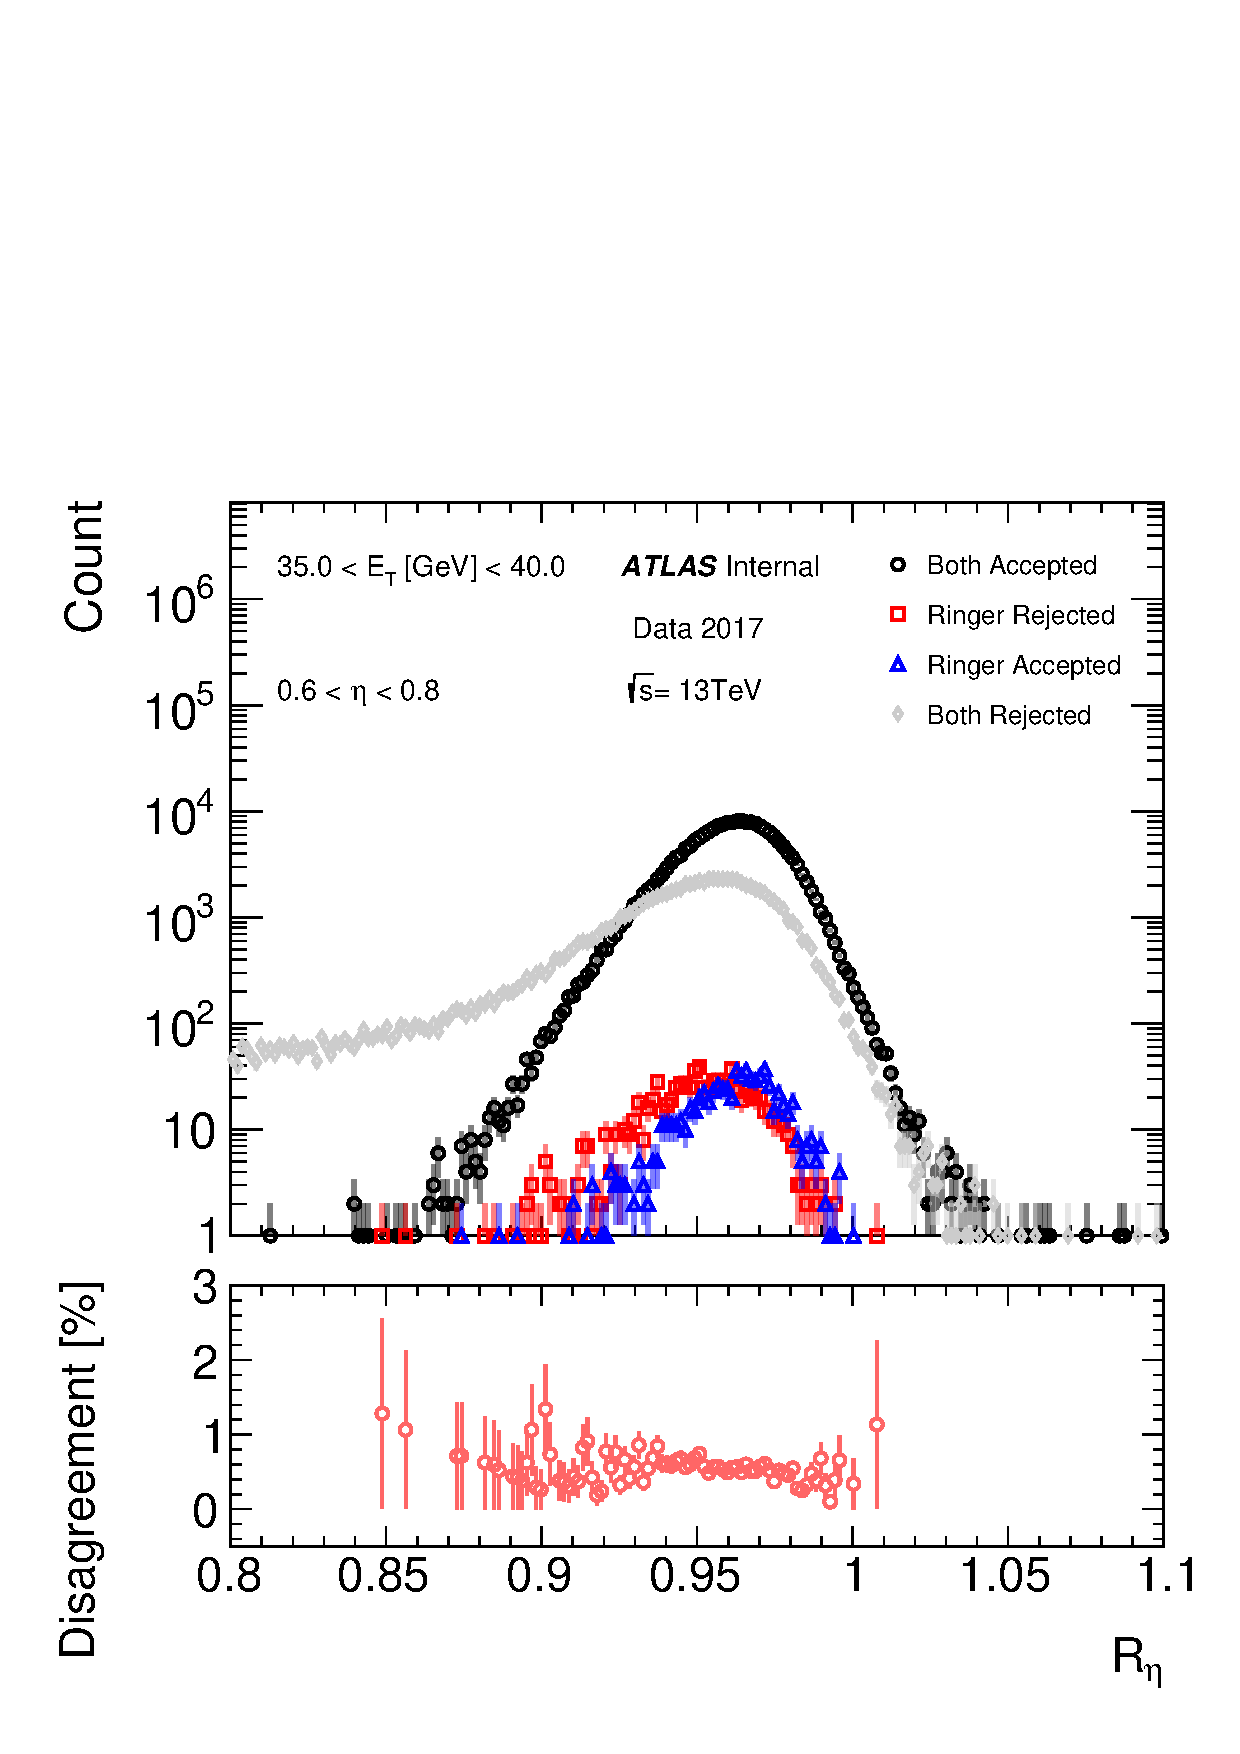
\includegraphics[width=\textwidth]{figures/quadrant_plots/reta.pdf}
\caption{}
\label{fig:quadrant_calo_variables_30GeV_eta}
\end{subfigure}
%\hfill
\begin{subfigure}[c]{.49\textwidth}
\centering
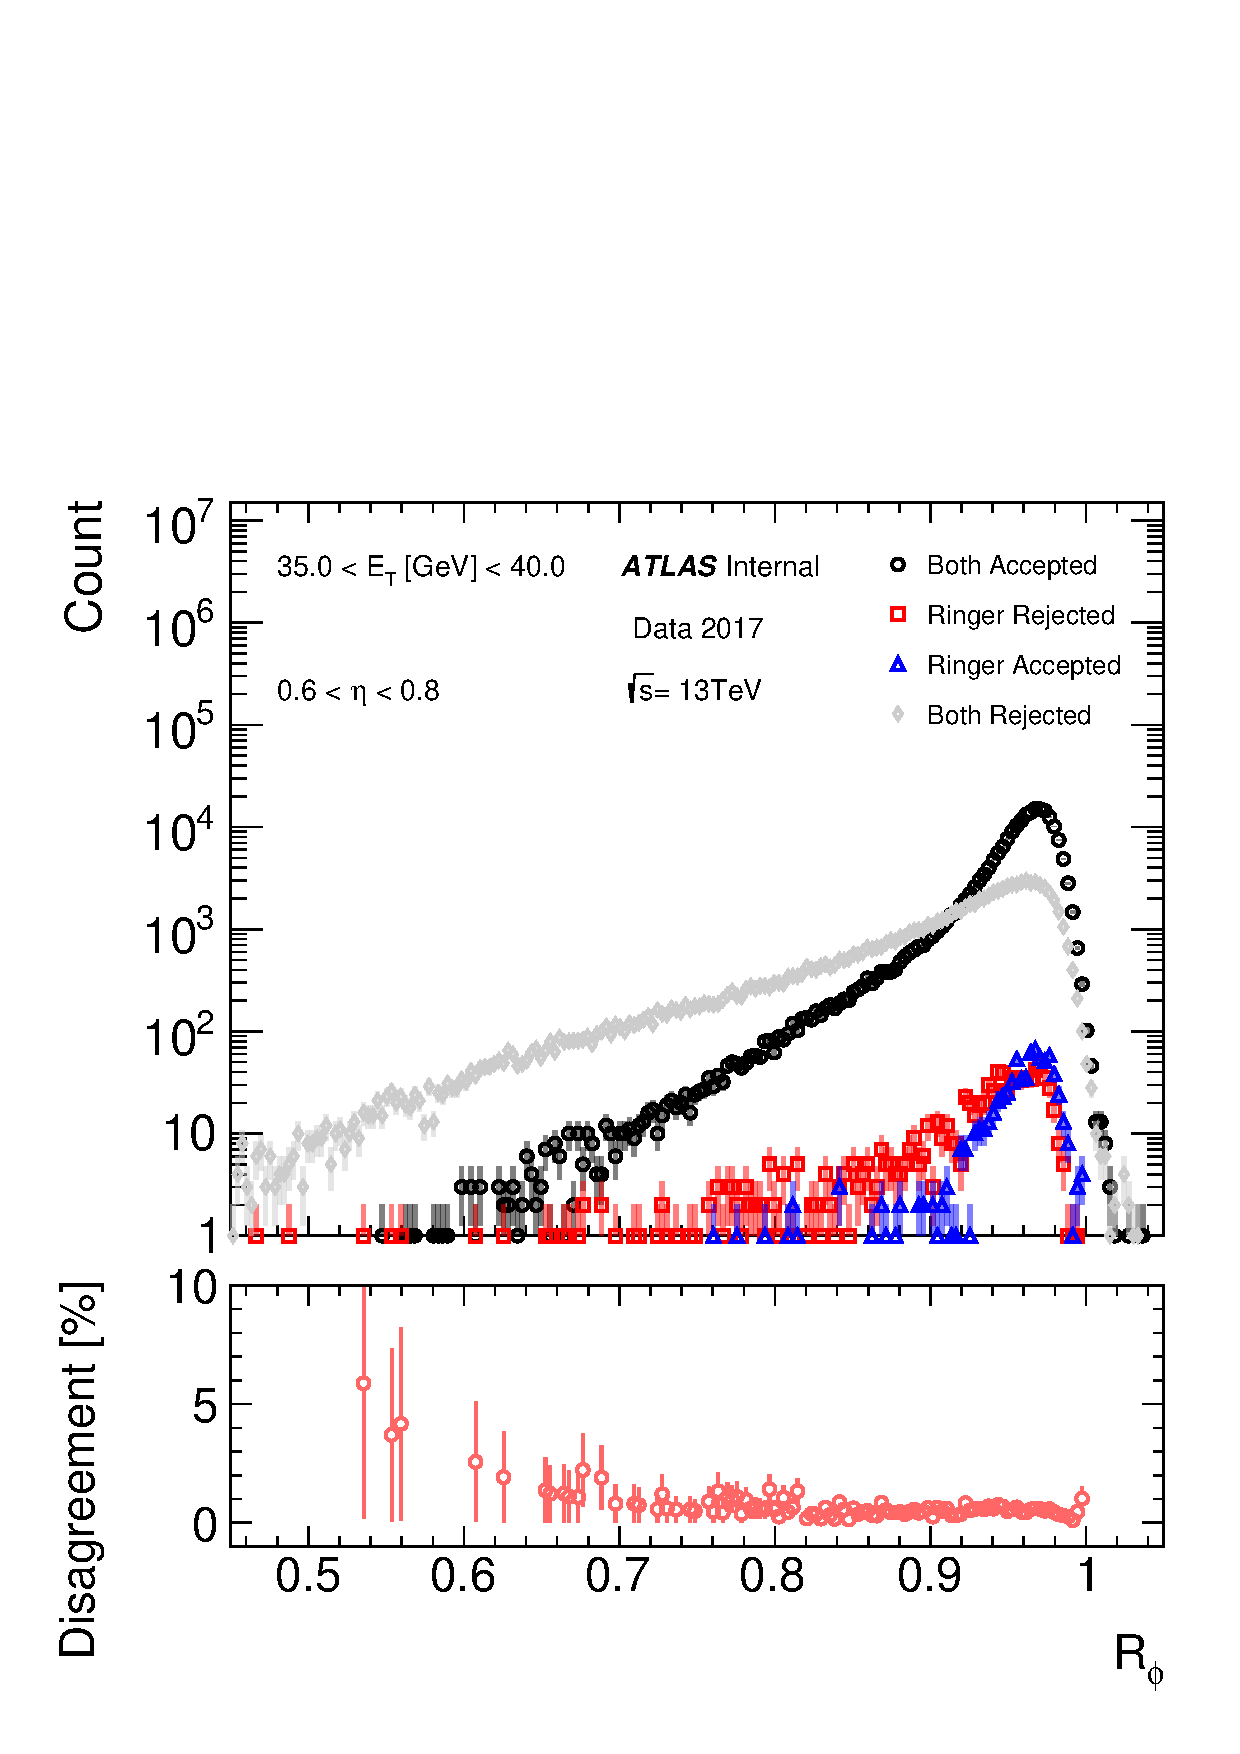
\includegraphics[width=\textwidth]{figures/quadrant_plots/rphi.pdf}
\caption{}
\end{subfigure} 
%\end{figure}
%\begin{figure}[p]\ContinuedFloat
\begin{subfigure}[c]{.49\textwidth}
\centering
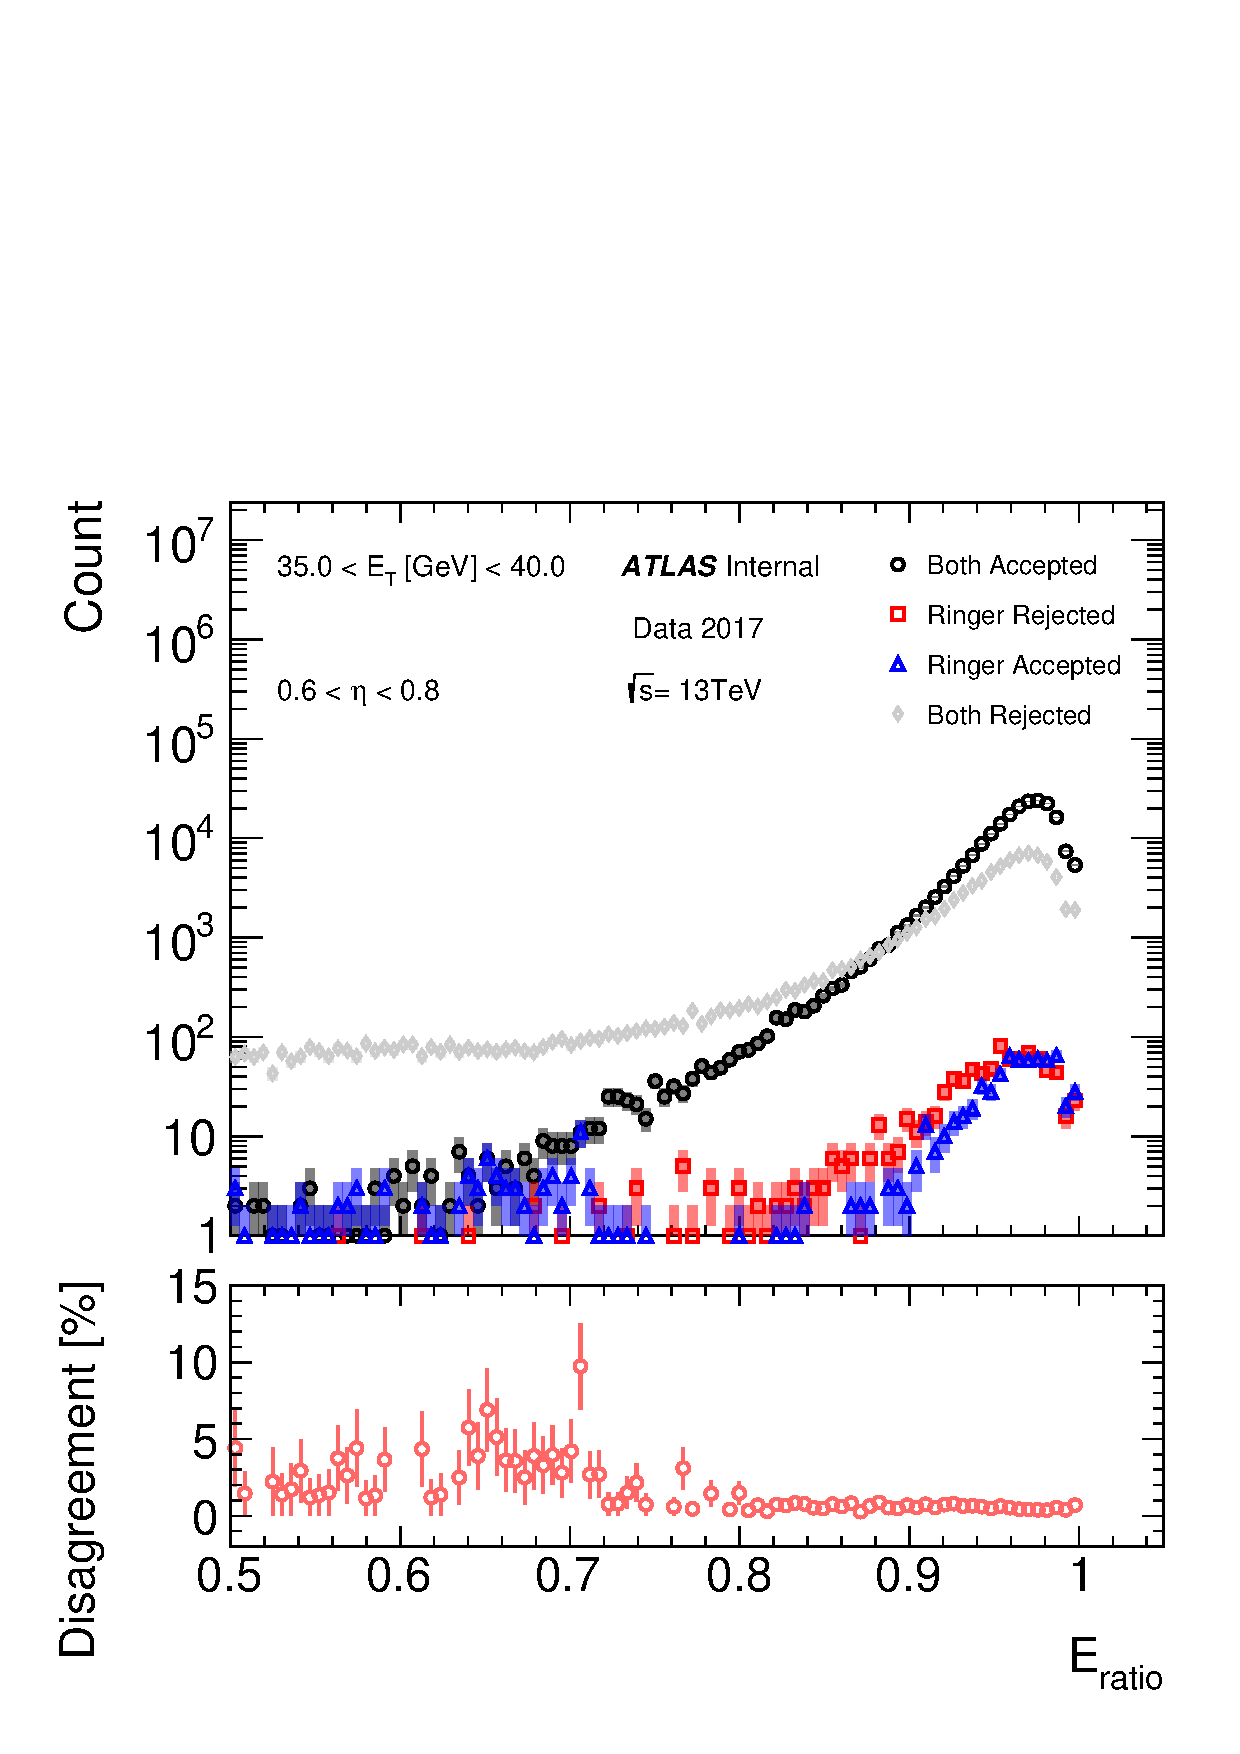
\includegraphics[width=\textwidth]{figures/quadrant_plots/eratio.pdf}
\caption{}
\end{subfigure}
\hfill
\begin{subfigure}[c]{.49\textwidth}
\centering
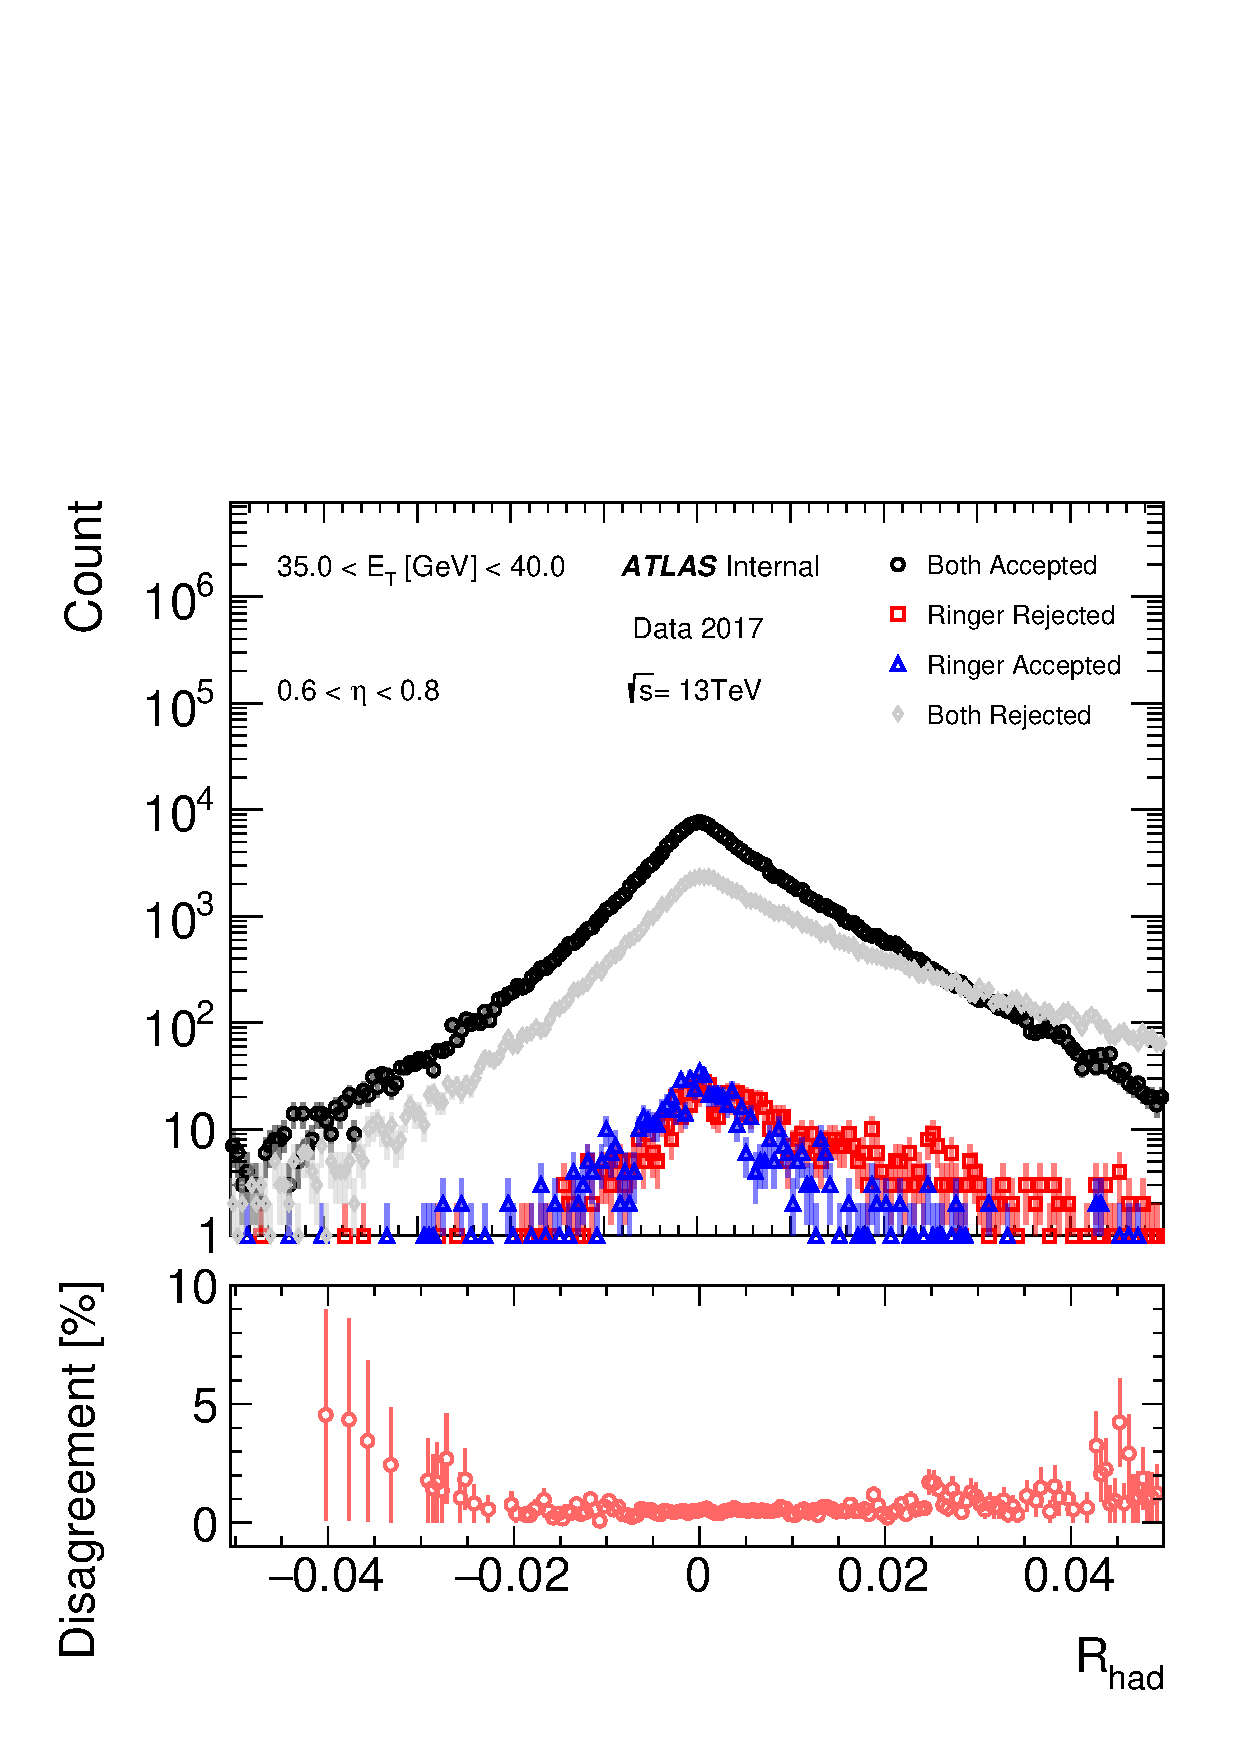
\includegraphics[width=\textwidth]{figures/quadrant_plots/rhad.pdf}
\caption{}
\end{subfigure} \\


\caption{\label{fig:quadrant_calo_variables_30GeV}
    Quadrant Analysis plots for a selection of shower-shape variables used in the offline electron identification algorithm for the $0.6<\abseta{}<0.8$ and $30<\et{}<35$~\GeV region. The top pad in each figure shows the raw number of candidates for the four mutually exclusive cases: accepted both with and without 
	the \rnn{} (black); accepted only with the \rnn{} (blue); accepted only with the Cut-based (red); rejected both with \rnn and with Cut-based (grey). The bottom pad shows 
	the disagreement as defined in Eq.~\eqref{eq:disagreement}. The absence of points of disagreement is due to the absence of events in the bins for the blue and red histogram cases.
}
%Quadrant analysis plots for the offline-reconstructed
%calorimetry variables employed in the
%likelihood and \wstot{} for the $0.6<\abseta{}<0.8$ and
%$30<\et{}~[\text{GeV}]<40$ slices.}%
\end{figure}


\begin{comment}
    
\begin{figure}[h!tb]
%\centering
%\begin{subfigure}[c]{.49\textwidth}
\centering
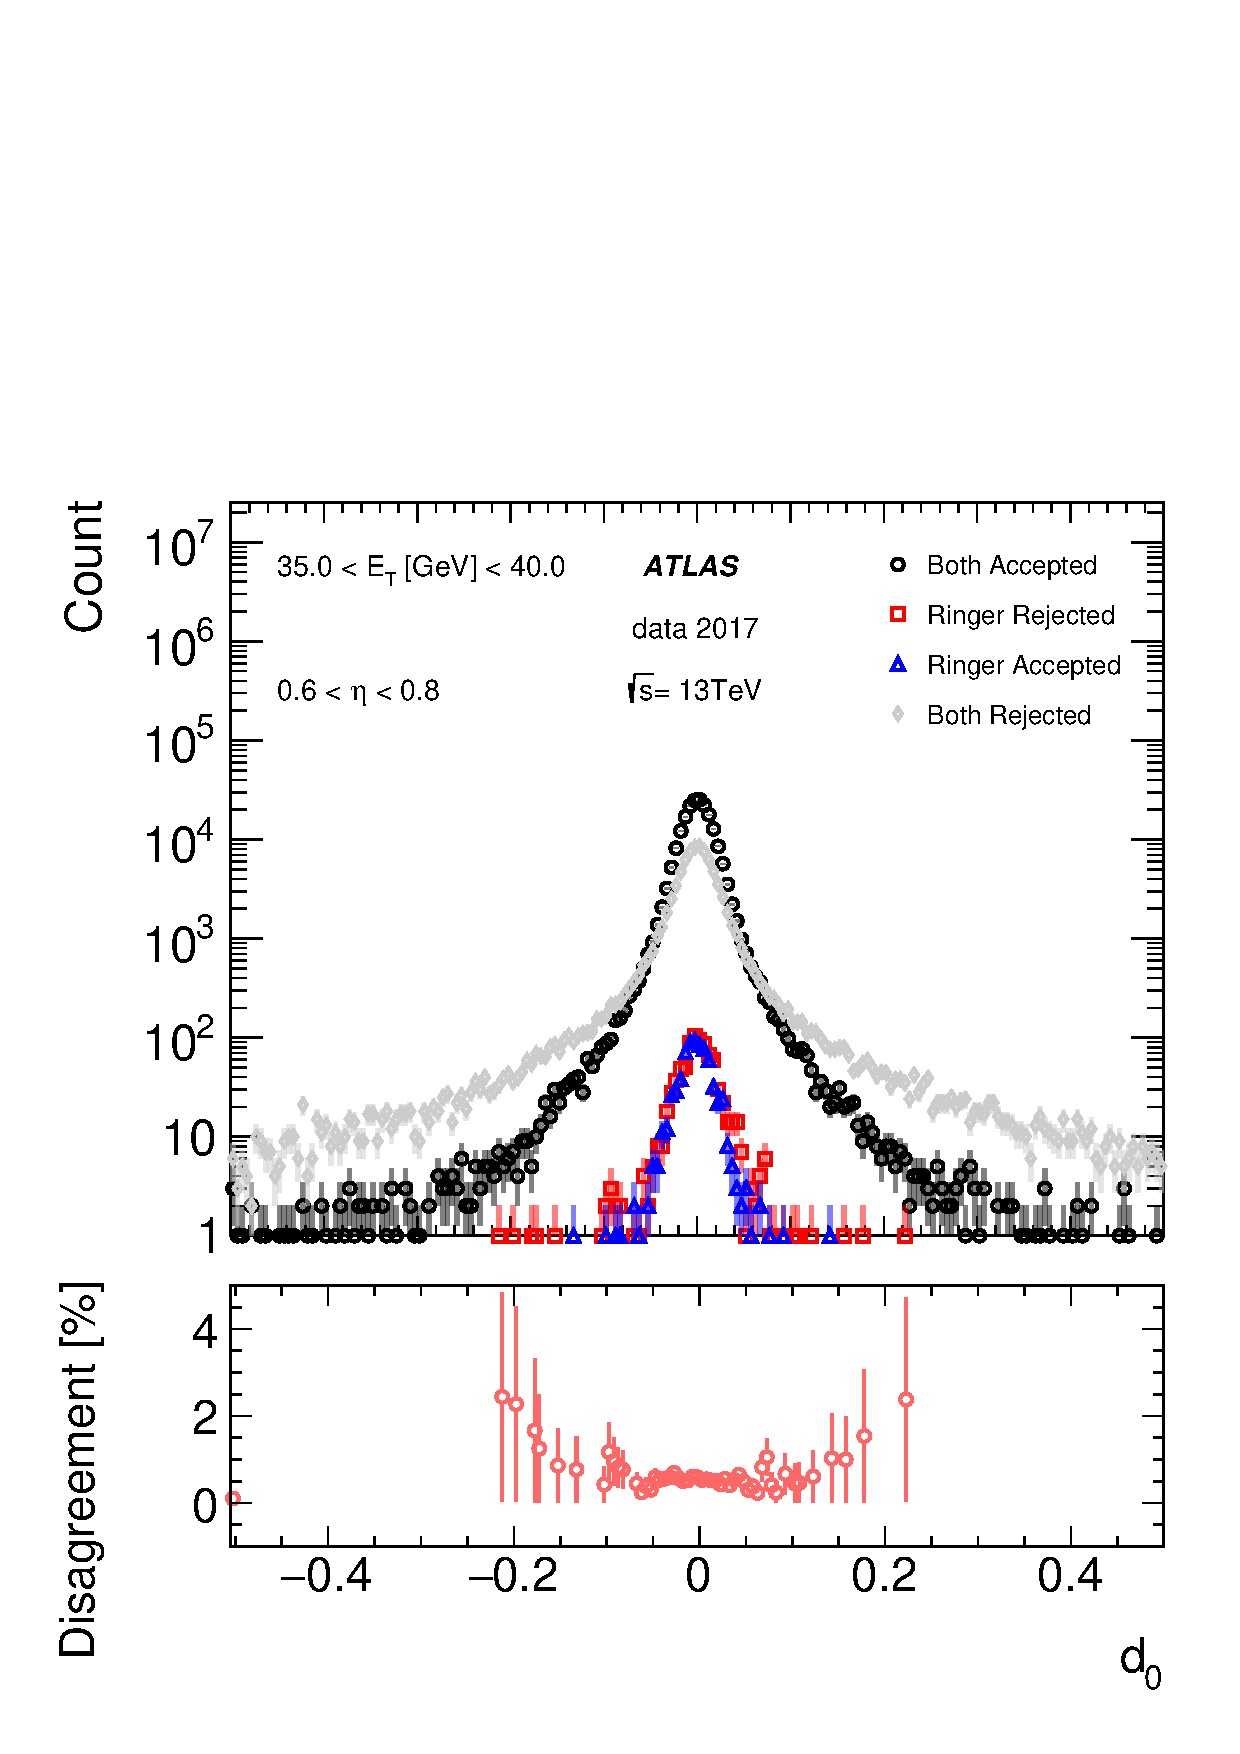
\includegraphics[width=.5\textwidth]{figures/quadrant_plots/d0.pdf}
\caption{\label{fig:quadrant_track_variables_30GeV}
Quadrant analyses plots for the offline-reconstructed ID variable $d_0$ employed in the
likelihood for the $0.6<\abseta{}<0.8$ and $35<\et{}~[\text{GeV}]<40$ slice. The variable $d_0$ is defined as the transverse parameter of the impact point with respect to the collision beam.
}
\end{figure}
\end{comment}






\FloatBarrier
\subsection[Homogeneity Tests]{Homogeneity Tests}\label{ssec:agreement}


The homogeneity tests evaluate the impact of using different trigger strategies—\rnn{}-based and cut-based—on the offline likelihood identification of tag electrons. To perform the study, a pair of duplicated single-electron triggers was used online. Both required $E_T >$ \SI{28}{\GeV}, the \enquote{tight} identification, and \enquote{loose} isolation criteria. One version incorporated the \rnn{}-based selection, while the other did not. The same offline identification criteria used in the likelihood optimization described in~\cite{PERF-2017-01} were applied throughout the analysis.

%In this analysis, the impact on the offline likelihood identification requirements of using different triggers, \rnn{} and cut-based, applied to the tag electron, is evaluated. 
%This study requires a pair of duplicated triggers, applying a HLT\_e28\_lhtight\_nod0\_(noringer)\_ivarloose trigger selection with and without the \rnn{} (noringer), operating together online. 
%The analysis is performed using the full 2017 collision dataset, selecting electron candidates with transverse energy above \SI{15}{\GeV}, and applying the same offline identification criteria used in the likelihood- based optimization described in \cite{PERF-2017-01}.

%The analysis is performed using the full 2017 collision data with the same selection as used for the offline likelihood optimization for electrons with \ET above \SI{15}{\GeV}~\cite{PERF-2017-01}.

%To benefit from the full 2017 dataset, collision data collected before TS1 were also employed. If the profiles of the calorimetry and track variables are statistically identical, the \rnn{} trigger is not expected to cause any relevant change in the derivation of the offline likelihood PDFs.  
%The statistical method for profile evaluation is described in Section~\ref{top:homogeneity_method} and the results are available in Section~\ref{top:agreement_homogeneity_results}.

%\subsubsection{Method}\label{top:homogeneity_method}

%The problem is addressed by applying homogeneity tests to histograms~\cite{homogeneity_test} in order to check for systematic effects of the trigger configuration. 
This analysis addresses this by applying homogeneity tests to histograms~\cite{homogeneity_test} to identify potential differences in the distributions of physics quantities arising from different trigger configurations.
These tests are based on a test originally developed by Pearson~\cite{pearson1911probability} and popularly employed in many fields beyond high-energy physics, e.g.\ social sciences~\cite{wickens2014multiway} and health~\cite{ma2015homogeneity}, where they are usually called contingency or consistency tests.

%In order to benefit from the tests without having to customize them to an ATLAS-specific analysis set-up, the collision data were split into two statistically independent groups or samples, consisting of data alternately taken from consecutive short time periods to keep their data-taking conditions as similar as possible. 

%The $p$-value, or probability value, is a measure used in statistical hypothesis testing to determine the significance of one's results. It represents the probability of obtaining an observed result if the null hypothesis (which states that there is no effect or no difference between the two trigger strategies) is true. By comparing the $p$-values of the two groups, it is possible to evaluate how the different configurations affect the likelihood that the profiles are being drawn from the same distribution. 
%If the $p$-values have negligible fluctuations with respect to the values obtained from tests comparing the same triggers, then the systematic effect in the profiles is negligible for a dataset that is half\footnote{Each group contains approximately half of the integrated luminosity.} of the size of the whole available dataset.

%\footnote{The p-value here is defined by: $P-value \approx f(x, k) = \frac{1}{2^{k/2}\Gamma(k/2)}x^{k/2 -1}e^{-x/2}$, where $x\in(0, \infty)$ and $k>0$}

%The $p$-value is the probability of obtaining results at least as extreme as those observed, assuming the null hypothesis is true. In this context, the null hypothesis states that there is no effect or no difference between the two trigger strategies. It represents the probability of observing a given result under this assumption. By comparing the $p$-values of the two groups, it is possible to evaluate how the different configurations influence the likelihood that the profiles are drawn from the same underlying distribution.


%To provide better insight into possible distortions, the corresponding  individual $\chi_{i,j}^{s}$ contributions, allowing them to assume positive or negative values by defining

To enable homogeneity tests without adapting them to ATLAS-specific setups, the 2017 collision data set was split into two statistically independent samples. These groups were constructed by alternating events taken at short time intervals to ensure similar data-taking conditions.

The $p$-value represents the probability of observing a result at least as extreme as the one measured, assuming the null hypothesis is true. In this case, the null hypothesis states that the distributions of the given variable are identical across the two samples. Comparing $p$-values across different samples helps assess whether the trigger configuration affects the shapes of the physics distributions.

To further investigate possible distortions introduced by the trigger algorithms, a bin-by-bin comparison is performed on histograms of shower-shape variables used in the offline electron identification. The signed $\chi$-value, defined in Equation~\ref{eq:signed_chi}, is used for this purpose. In this expression, $r_{i,j}$ and $b_{i,j}$ are the event counts in the $j^\text{th}$ bin and $i^\text{th}$ $\et{}\times\abseta{}$ region, collected by the group using the trigger with and without the \rnn{}, respectively. This equation quantifies the deviation between the two trigger configurations and allows both positive and negative contributions to be visualized.

\begin{equation}
  \chi_{i,j}^{s} = \frac{(r_{i,j} - b_{i,j})}{\sqrt{b_{i,j}}},
  \label{eq:signed_chi}
\end{equation}


\subsubsection{Results}\label{top:agreement_homogeneity_results}




Regardless the trigger configuration, the homogeneity tests between the two groups result in similar $p$-values. %In other words, the fluctuations in the profiles are mainly statistical, with no sign of systematic effects due to the trigger configuration. 
The comparison of shower-shape distributions between the two statistically independent groups reveals fluctuations consistent with statistical uncertainty. No significant deviations are observed that would indicate systematic differences arising from the trigger configuration

Figure~\ref{fig:groups_homogeneity_calo} shows the residuals (bottom) for the \reta, \rphi, \eratio, and \rhad calorimetry variables when the reference histogram is obtained from collision data collected by the trigger without the \rnn{} for the first group (top). The residuals are dominated by statistical fluctuations (i.e., the residual values fluctuate around a central value) and are within expectations under the homogeneity hypothesis for most variables and regions. Similar behavior is observed for track variables. 

\begin{figure}[h!]
\begin{center}
\begin{subfigure}[c]{.48\textwidth}
\centering
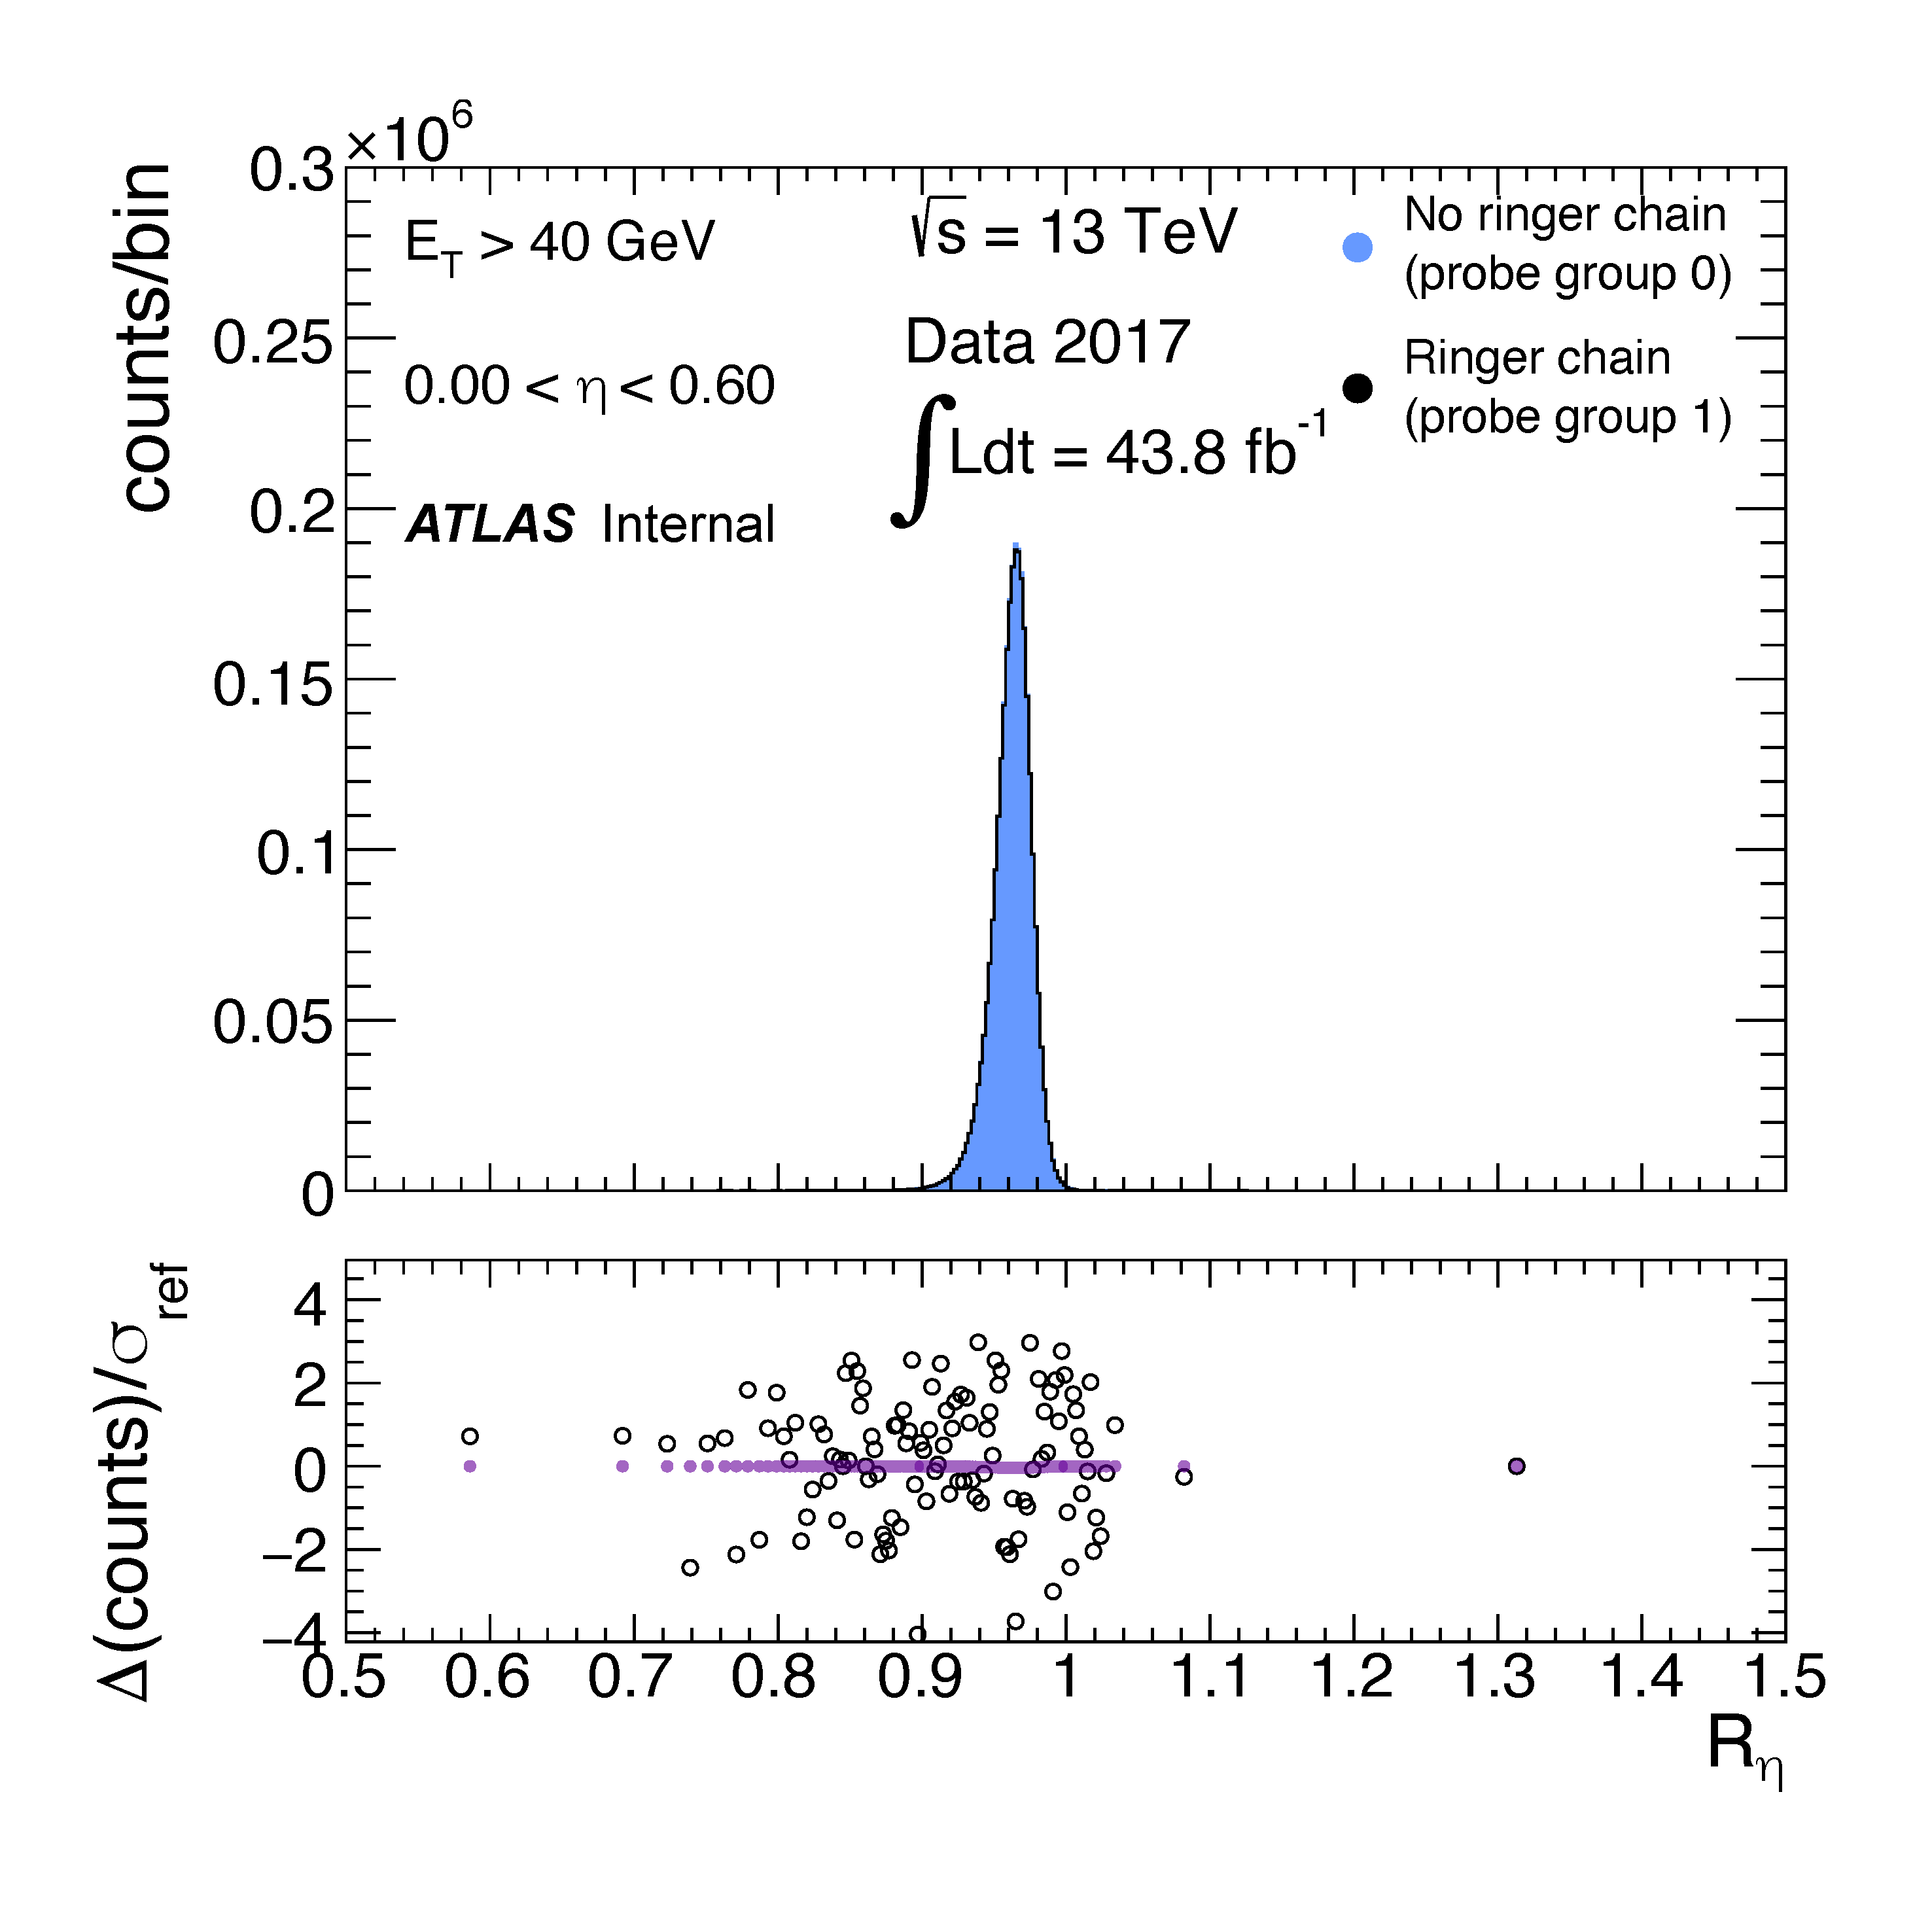
\includegraphics[width=\textwidth]{figures/noAdjustment/el_reta_et40eta0_00_sigma_base_new.pdf}
\caption{}%

\end{subfigure}
\hfill
\begin{subfigure}[c]{.48\textwidth}
\centering
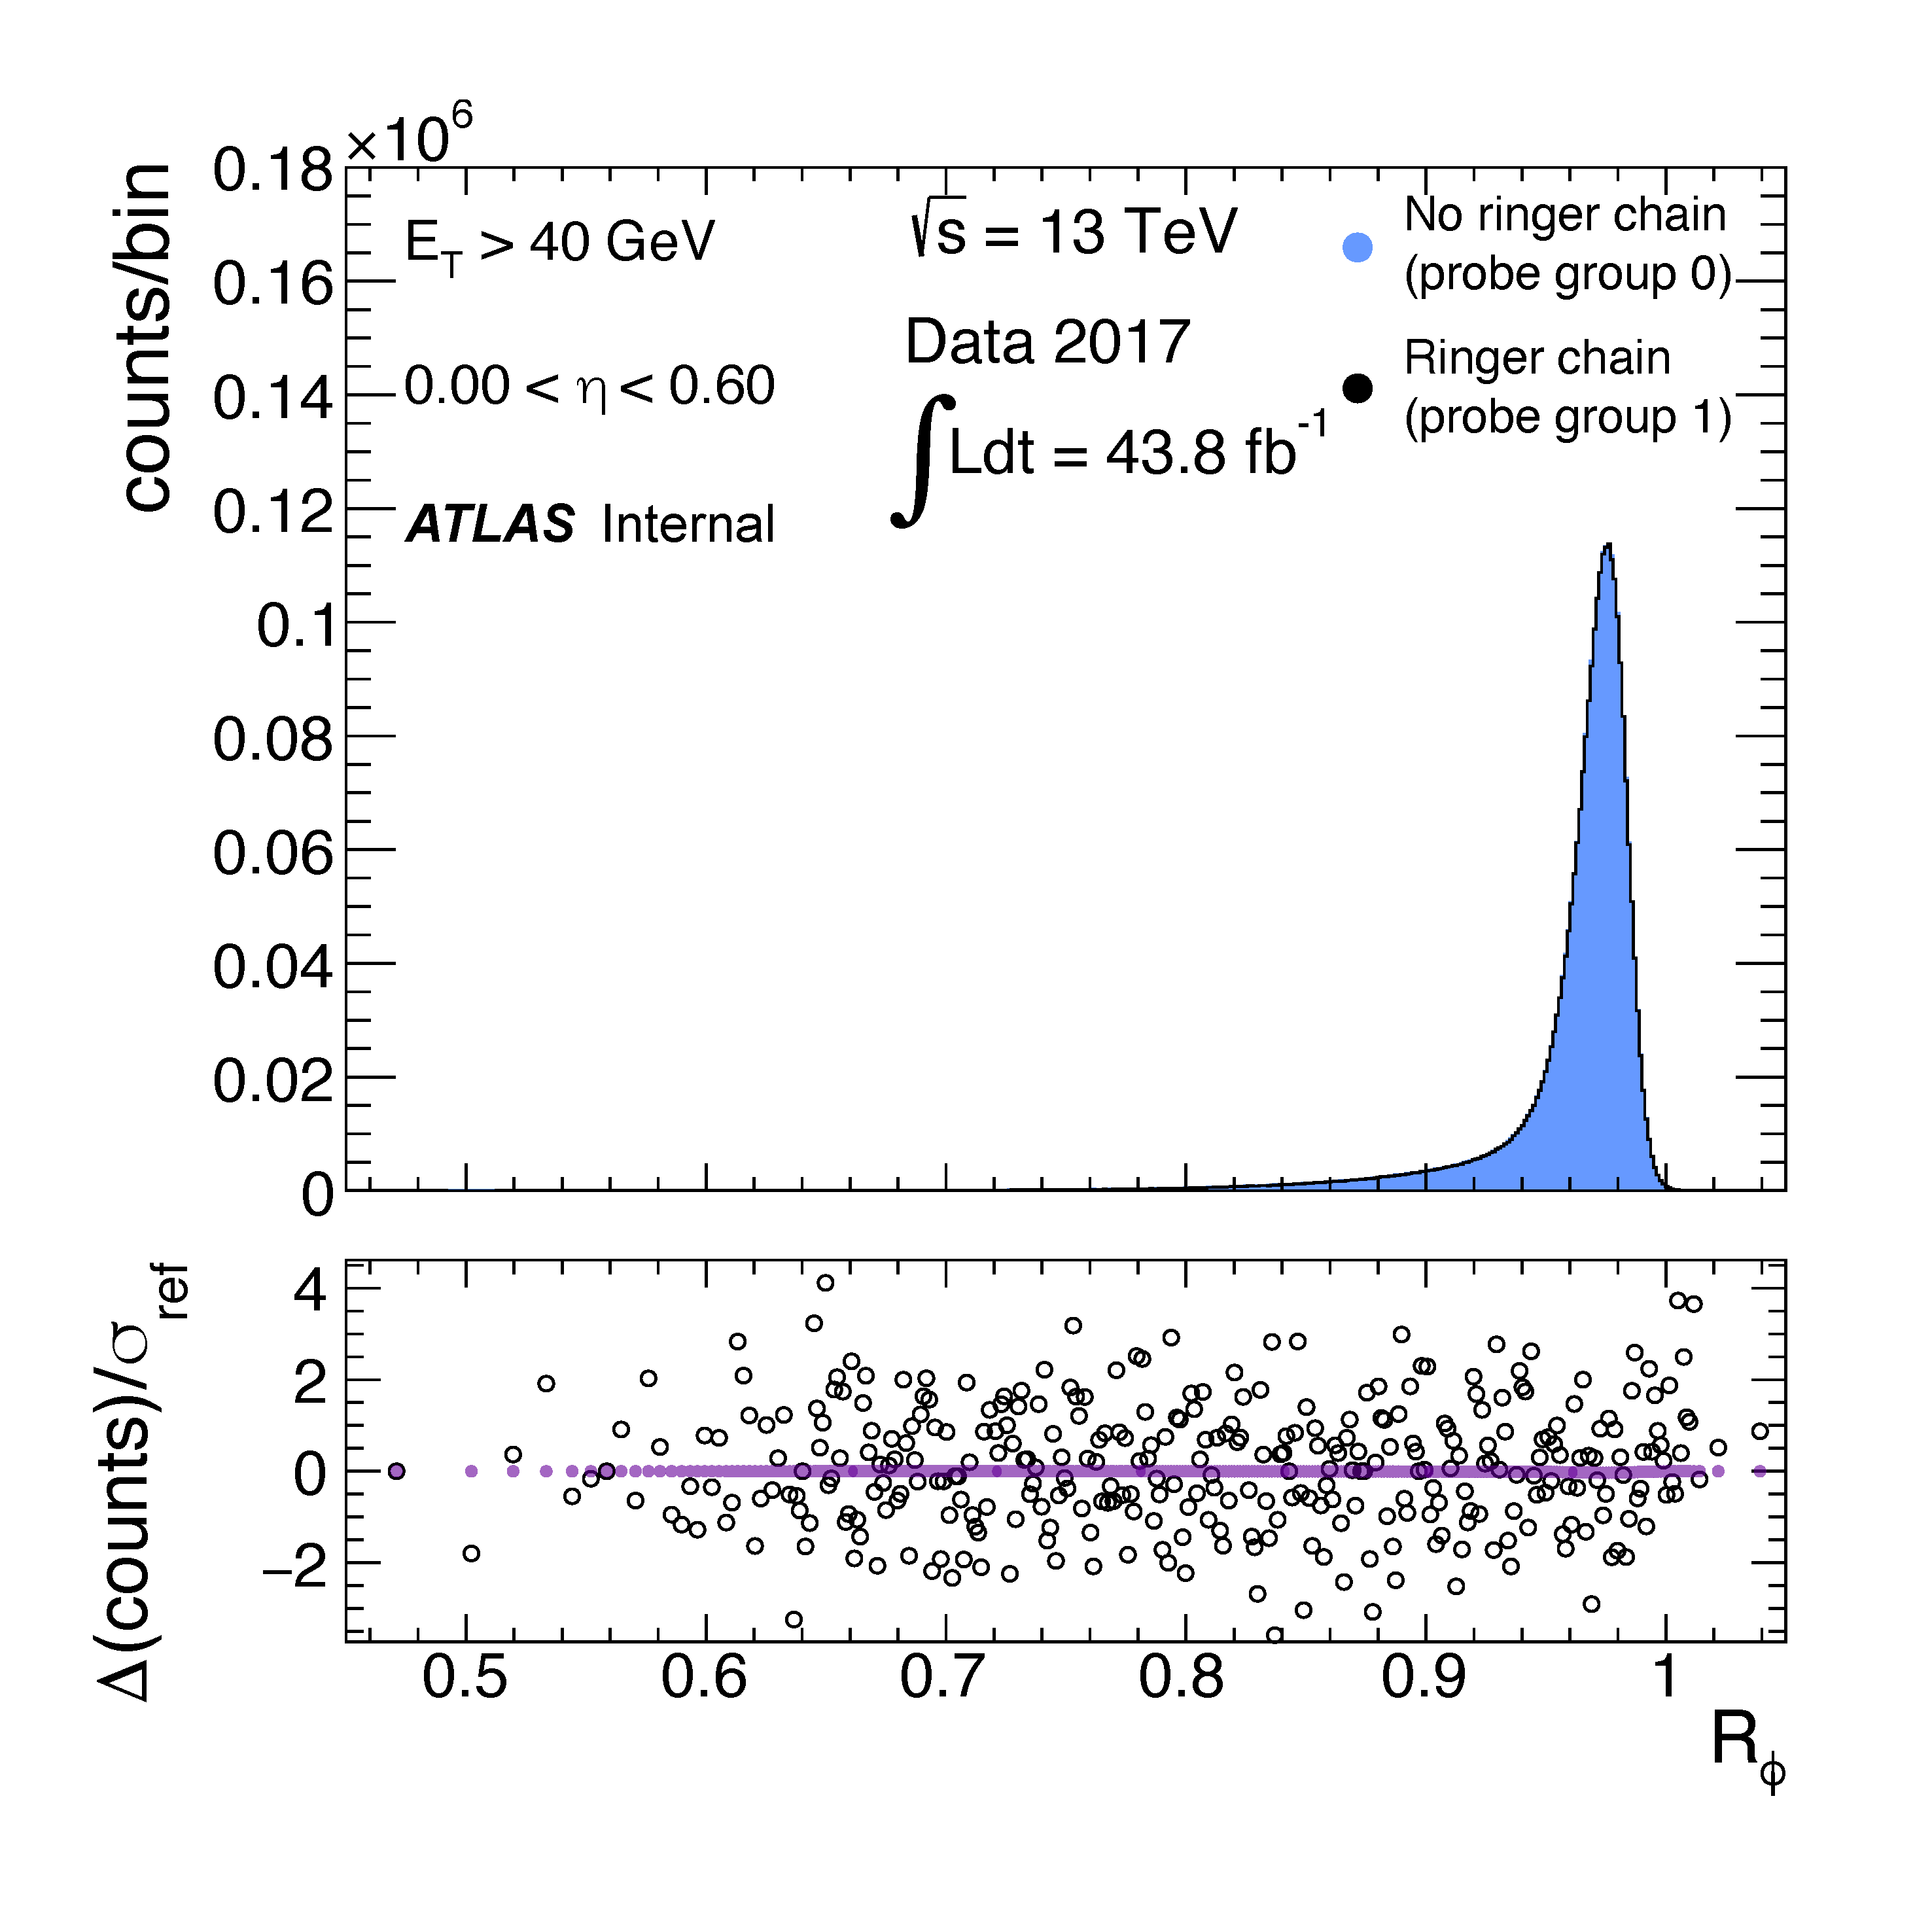
\includegraphics[width=\textwidth]{figures/noAdjustment/el_rphi_et40eta0_00_sigma_base_new.pdf}
\caption{}%

\end{subfigure} \\
\begin{subfigure}[c]{.48\textwidth}
\centering
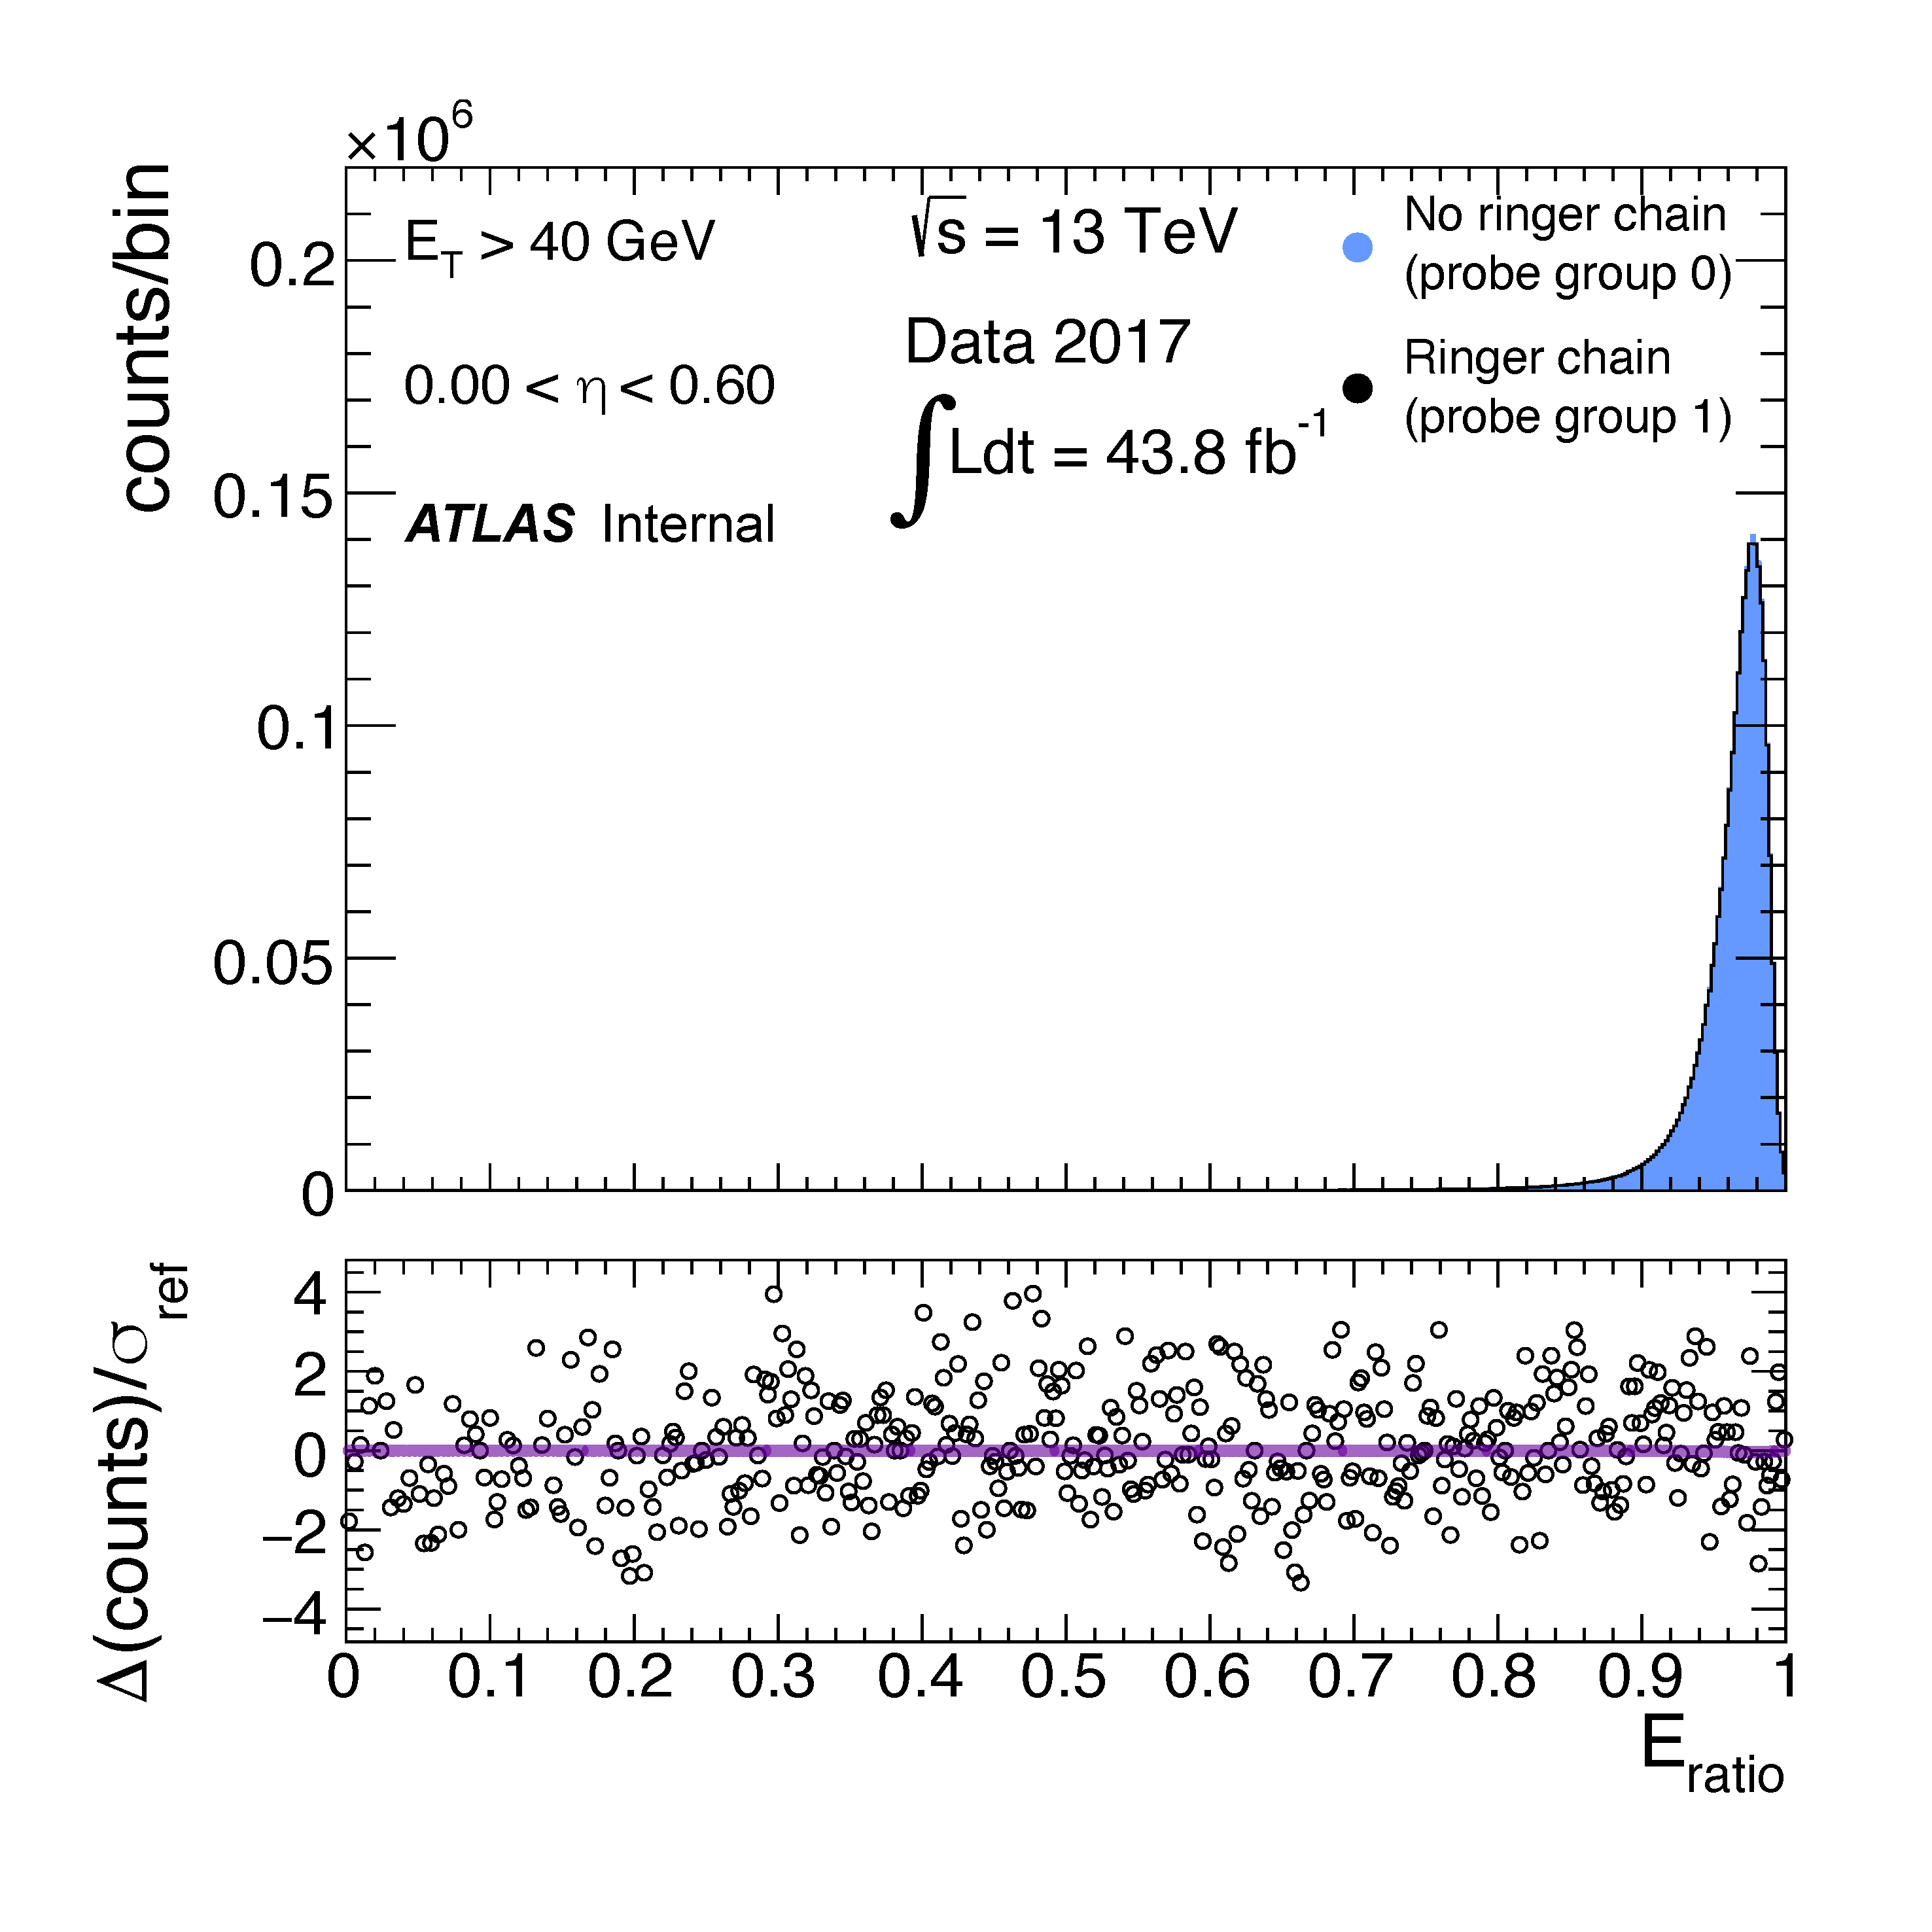
\includegraphics[width=\textwidth]{figures/noAdjustment/el_eratio_et40eta0_00_sigma_base_new.pdf}
\caption{}%

\end{subfigure}
\hfill
\begin{subfigure}[c]{.48\textwidth}
\centering
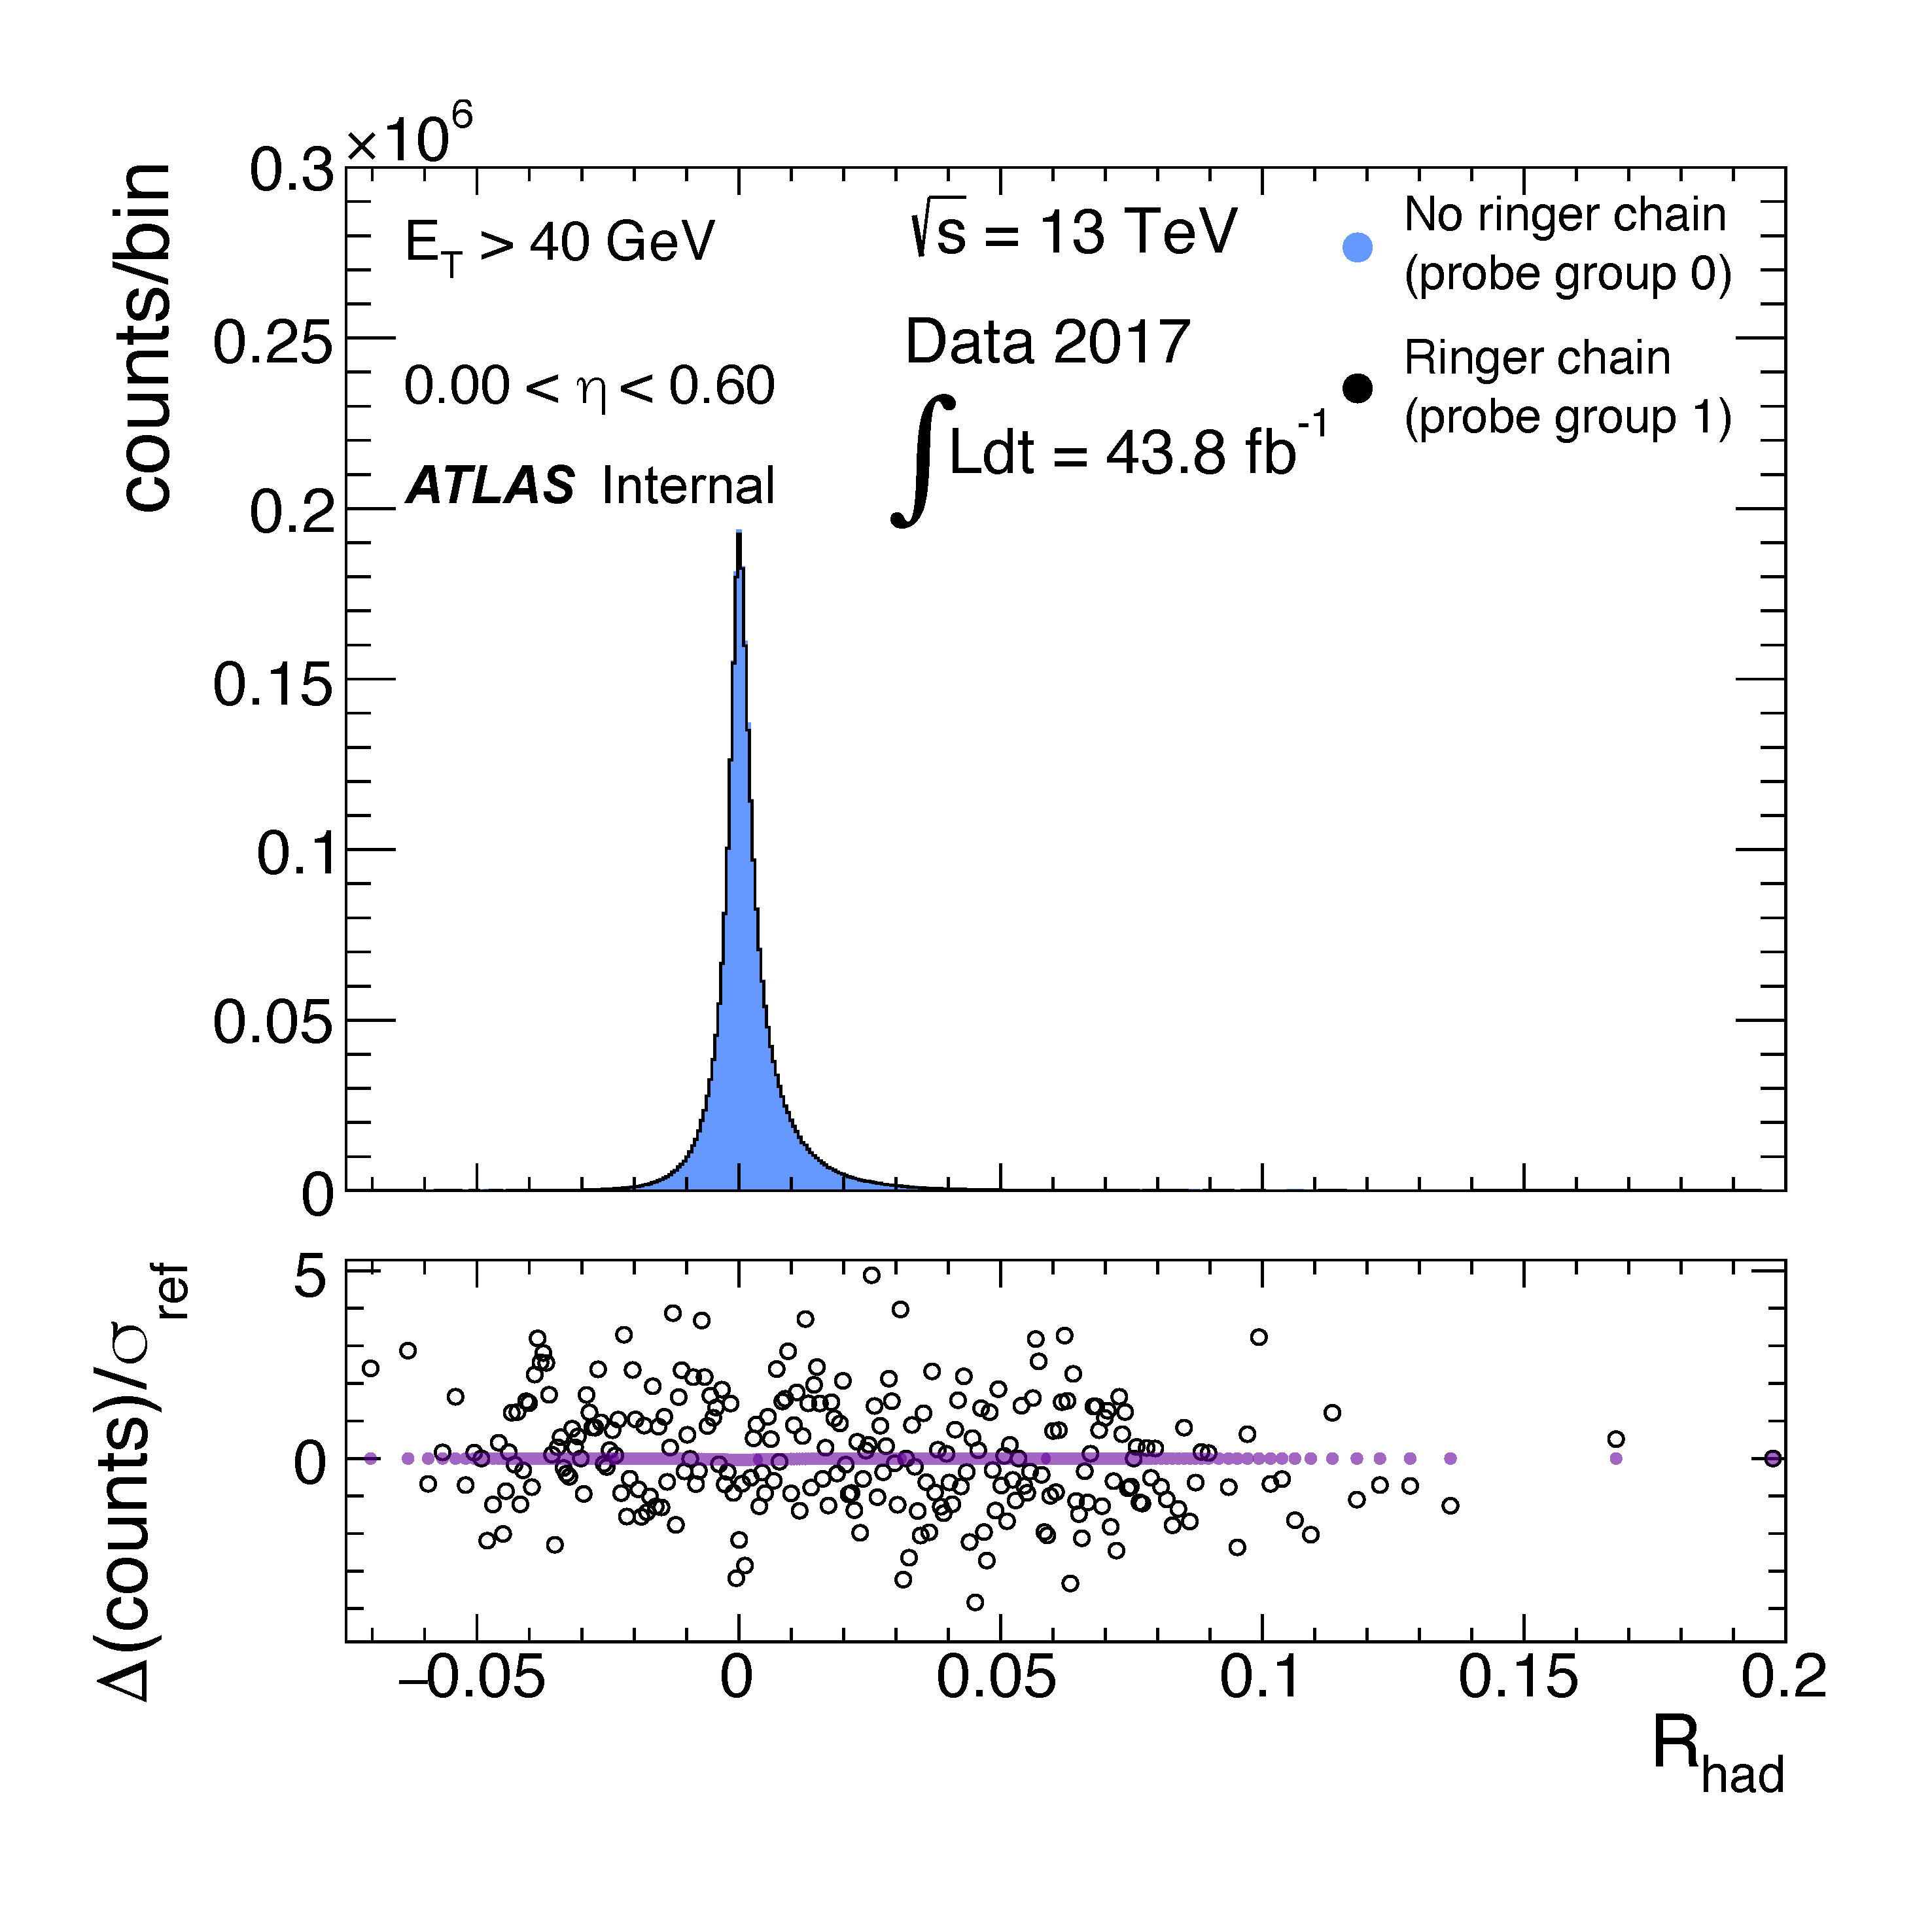
\includegraphics[width=\textwidth]{figures/noAdjustment/el_rhad_et40eta0_00_sigma_base_new.pdf}
\caption{}%

\end{subfigure} \\
\caption{%
\textbf{Top:} Profile histograms of the \reta, \rphi, \eratio, and \rhad calorimetry variables used in the offline likelihood selection, shown for the $\et>\SI{40}{\GeV}$ and $0.0<\abseta{}<0.8$ region. The distributions are obtained from two statistically independent data samples: one collected using the cut-based selection (blue area histogram), and the other using the trigger with the \rnn{} (black line histogram). The assignment of trigger type to group is arbitrary and alternated across time intervals to ensure statistical independence.
\textbf{Bottom:} Bin-by-bin residuals computed using the signed $\chi^s$ statistic (black circles, see Eq.~\ref{eq:signed_chi}), which quantify the deviation between the two trigger configurations. The horizontal line at zero (purple dots) serves as a visual reference indicating no deviation.
}
%	Top: Profile histograms for the \reta, \rphi, \eratio, and \rhad calorimetry variables employed 
%	in the offline likelihood in the $\et>\SI{40}{\GeV}$ and $0.0<\abseta{}<0.8$ regions using 
%	collision data collected by triggering without the \rnn{} in the first arbitrary data group
%	(blue area histogram) and collision data collected by triggering with the \rnn{} in the second
%	arbitrary data group (black line histogram).  Bottom: residual contributions using 
%	the $\chi^s$ statistic (black circles, from Eq.~(\ref{eq:signed_chi})), and the expected
%	$\chi^s$ residuals if there are no distortions or statistical fluctuations with respect to the
%	reference (purple dots at zero).
%
\label{fig:groups_homogeneity_calo}
\end{center}
\end{figure}%


\FloatBarrier
